% File: org_classi.tex
% Created: 2014-12-05
% Author: Tesser Paolo
% Email: p.tesser921@gmail.com
% 
%
% Modification History
% Version	Modifier Date	Author			Change
% ====================================================================
% 0.0.1	2014-12-05	Tesser-Paolo		inserita sezione 
% ====================================================================
% 0.0.2	2014-12-05	Tesser Paolo		iniziata stesura
%

\section{Organizzazione strutturale delle classi}
La struttura dell'applicativo è composta da diversi package, con all'esterno di essi la classe \textbf{PuzzleSolver} responsabile dell'esecuzione del programma e dell'istanziazione delle classi in oggetti per risolvere il puzzle. \\
Anche se tutte le classi all'interno di questi package lavorano bene assieme e tra loro esistono alcune dipendenze, si è deciso di tenere un minimo si separazione logica per le diverse componenti. \\
Nei sotto capitoli seguenti  verranno illustarti i package utilizzati e le classi presenti in essi.

	\subsection{Puzzle}
TO DO

	\subsection{Solver}
TO DO
	
	\subsection{FileInputOutput}
		\begin{figure}[htbp]
			\centering
			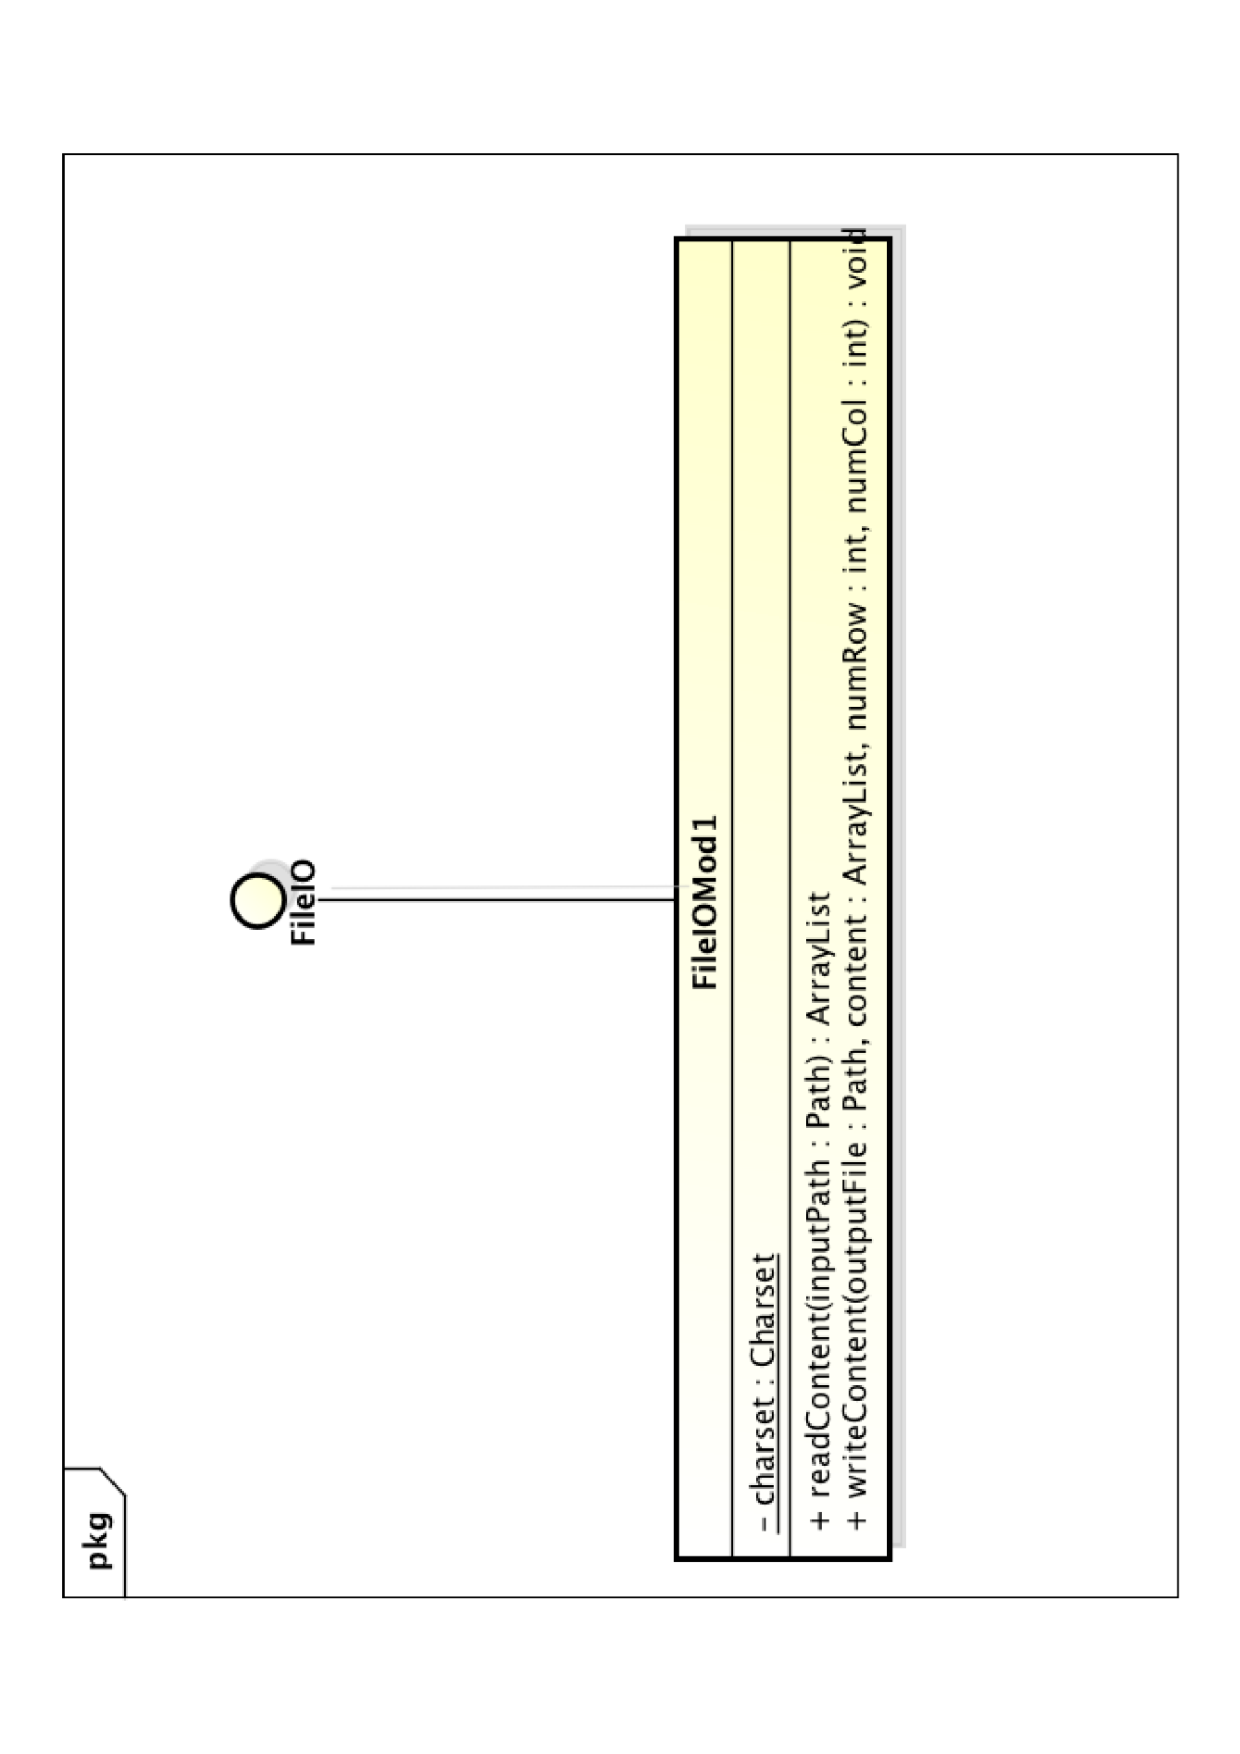
\includegraphics[width=15cm]{img/FileInputOutput.pdf}
			\caption{Package FileInputOutput}
			\label{Package FileInputOutput}
		\end{figure}
TO DO
	
